\newpage
\section{Theoretical Analysis and Control Design}

\subsection{Space-State Formulation}

\par The non-linear dynamics of the system imply that it needs to be linearized around an equilibrium point, which, given the objective of this report, is the unstable equilibrium where the pendulum is in the upright vertical position. 
This equilibrium corresponds to all state variables being equal to zero. The derivation of the non-linear model and the subsequent 
linearization are not the focus of this report and can be found in Chapter 2 of Samuel Balula's thesis \cite{balula2016inverted}.  
The linearized model of the system, which reasonably represents the dynamics, is given by:

\vspace{1pt}
\[
\begin{cases}
\mathbf{\dot{x}} = A \mathbf{x} + B \mathbf{u} \\
\mathbf{y} = C \mathbf{x} + D \mathbf{u}
\end{cases}
\]
\vspace{1pt}

\par where $\mathbf{x} = [\alpha \ \dot{\alpha} \ \beta \ \dot{\beta} \ i]^T$ is the 5-dimensional state vector, and $i$ is the motor current. The one-dimensional input vector $\mathbf{u} = u$ corresponds to the DC voltage, in \textit{Volts}, applied to the terminals of the DC motor through a power amplifier, directly controlling $\alpha$. The output vector $\mathbf{y} = [\alpha \ \beta]^T$ consists of the sensor measurements, corresponding to the angular positions of the arm and the pendulum, respectively.

\par The system matrices $A$, $B$, $C$, and $D$ are given by:


\[
A =
\begin{bmatrix}
    0 & 1 & 0 & 0 & 0 \\
    0 & -0.0174 & 20.7861 & -0.0023 & 57.5344 \\
    0 & 0 & 0 & 1 & 0 \\
    0 & -0.0174 & 63.8319 & -0.0071 & 57.4388 \\
    0 & -232.0252 & 0 & 0 & -755.425
\end{bmatrix}
\]
\[
B = 
\begin{bmatrix} 0 \\ 0 \\ 0 \\ 0 \\ 333.3 \end{bmatrix}, \quad
C = 
\begin{bmatrix} 1 & 0 & 0 & 0 & 0 \\ 0 & 0 & 1 & 0 & 0 \end{bmatrix}, \quad
D = 
\begin{bmatrix} 0 \\ 0 \end{bmatrix}
\]
\subsection{State-Space Analysis}

\par In this section, we analyze the previously formulated state-space model in terms of system poles, controllability, observability, and frequency response.
\\
\subsubsection{Q1 - System Poles}

\par The system poles are the eigenvalues of the dynamics matrix $A$. Using MATLAB's \texttt{eig()} function, the following poles were obtained:

\begin{table}[h]
\centering
\caption{Características dos Modos do Sistema}
\footnotesize
\renewcommand{\arraystretch}{1.3}
\setlength{\tabcolsep}{7pt}
\begin{tabular}{ccc}
\toprule
Polos & $\omega$ (rad/s) & $\tau$ (s) \\
\midrule
$0$ & 0 & $\infty$ \\
$-737.3$ & $7.37 \times 10^{2}$ & $1.36 \times 10^{-3}$  \\
$-19.36$ & $1.94 \times 10^{1}$ & $5.16 \times 10^{-2}$  \\
$-5.761$ & $5.76$ & $1.74 \times 10^{-1}$ \\
$\ \ 6.997$ & $7.00$ & $-1.43 \times 10^{-1}$  \\
\bottomrule
\end{tabular}
\label{modos_sistema}
\end{table}


\par Analysis of the poles shows that the system has three stable modes: two correspond to the mechanical damping of the pendulum, $\lambda_3 = -19.3673$ and $\lambda_4 = -5.7612$, and a very fast mode associated with the motor current, $\lambda_2 = -737.3184$. Additionally, the state $\alpha$ generates a pole at the origin, $\lambda_1 = 0$, due to being an integrator. This implies that after a perturbation, $\alpha$ will accumulate error over time without diverging or converging, reflecting the fact that the arm rotates without friction and does not naturally settle to an equilibrium. 

\par The single unstable mode, $\lambda_5 = 6.9974$, is related to the vertical pendulum position, which is the primary state we aim to control.
\\
\subsubsection{Q2 - Controllability}

\par A system is controllable if it is possible to transition from any state $x_1$ to another arbitrary state $x_2$ by applying an input $u(t)$ over a finite time interval. Knowing whether the system is controllable is crucial for understanding the limitations of the controller.

\par The controllability matrix is defined as:
\begin{equation}
\mathcal{C} = \begin{bmatrix} B & AB & A^2B & \cdots & A^{n-1}B \end{bmatrix},
\end{equation}
where $n$ is the number of states. Using MATLAB's \texttt{ctrb(A,B)} function, we obtained:

\[
\mathcal{C} =
\begin{bmatrix}
0 & 0 & 1.918 \times 10^{4} & -1.449 \times 10^{7} & 1.069 \times 10^{10} \\
0 & 1.918 \times 10^{4} & -1.449 \times 10^{7} & 1.069 \times 10^{10} & -7.881 \times 10^{12} \\
0 & 0 & 1.915 \times 10^{4} & -1.446 \times 10^{7} & 1.067 \times 10^{10} \\
0 & 1.915 \times 10^{4} & -1.446 \times 10^{7} & 1.067 \times 10^{10} & -7.869 \times 10^{12} \\
3.333 \times 10^{2} & -2.518 \times 10^{5} & 1.858 \times 10^{8} & -1.370 \times 10^{11} & 1.010 \times 10^{14}
\end{bmatrix}
\]

\par The system is controllable if the rank of the controllability matrix equals the number of states. Using MATLAB's \texttt{rank()} function, we obtained $\text{rank}(\mathcal{C}) = 5$, which equals the number of states. Therefore, the system is controllable.
\\
\subsubsection{Q3 - Observability}

\par A system is observable if, for any initial state $x(0)$, knowledge of the input $u(t)$ and output $y(t)$ over a finite time interval uniquely determines $x(0)$. Although the system is controllable, implementing a state-feedback controller requires knowledge of the full state\footnote{State-feedback control requires knowledge of the full state since the control law $u(t) = -Kx(t)$ explicitly depends on the state vector. In this project, an estimator was designed to reconstruct the state, resulting in the control law $u(t) = -K\hat{x}(t)$. State estimation is only possible if the system is observable, making observability a prerequisite for implementing state-feedback control when the state is not directly measurable.}. Since the state is not directly measurable, it must be reconstructed from the outputs, which is only possible if the system is observable.

\par The observability matrix is defined as:
\begin{equation}
\mathcal{O} = 
\begin{bmatrix}
C \\
CA \\
CA^2 \\
\vdots \\
CA^{n-1}
\end{bmatrix}
\end{equation}

\par Using MATLAB's \texttt{obsv()} function, the observability matrix was calculated as:

\begin{equation}
\mathcal{O} =
\begin{bmatrix}
1 & 0 & 0 & 0 & 0 \\
0 & 0 & 1 & 0 & 0 \\
0 & 1 & 0 & 0 & 0 \\
0 & 0 & 0 & 1 & 0 \\
0 & -1.740 \times 10^{-2} & 2.079 \times 10^{1} & -2.316 \times 10^{-3} & 5.753 \times 10^{1} \\
0 & -1.738 \times 10^{-2} & 6.383 \times 10^{1} & -7.114 \times 10^{-3} & 5.744 \times 10^{1} \\
0 & -1.335 \times 10^{4} & -5.096 \times 10^{-1} & 2.079 \times 10^{1} & -4.346 \times 10^{4} \\
0 & -1.333 \times 10^{4} & -8.152 \times 10^{-1} & 6.383 \times 10^{1} & -4.339 \times 10^{4} \\
0 & 1.008 \times 10^{7} & -2.762 \times 10^{5} & 3.027 \times 10^{1} & 3.207 \times 10^{7} \\
0 & 1.007 \times 10^{7} & -2.729 \times 10^{5} & 2.960 \times 10^{1} & 3.202 \times 10^{7}
\end{bmatrix}
\end{equation}

\par Applying the \texttt{rank()} function shows that $\text{rank}(\mathcal{O}) = 5$, which equals the number of states. Therefore, the system is observable.
\vspace{1.5cm}
\subsubsection{Q4 - Bode Plots}
\par To evaluate the frequency response of the system, the transfer functions of $\alpha$ and $\beta$ relative to the input $u$ were determined, resorting to the function \texttt{ss2tf()}:

\begin{equation}
    \frac{\alpha(s)}{u(s)} = \frac{
1.92\times 10^{4}\, s^2 + 92.07\, s - 8.26\times 10^{5}
}{
s^5 + 755.45\, s^4 + 1.33\times 10^{4}\, s^3 - 4.82\times 10^{4}\, s^2 - 5.76\times 10^{5}\, s
}
\end{equation}

\begin{equation}
    \frac{\beta(s)}{u(s)} = \frac{
0.1915\,s^2
}{
s^5 + 755.45\, s^4 + 1.33\times 10^{4}\, s^3 - 4.82\times 10^{4}\, s^2 - 5.76\times 10^{5}\, s
}
\end{equation}

\par With the above transfer functions, we generated the Bode plots to characterize their frequency response.

\begin{figure}[htbp]
    \centering
    \begin{subfigure}[b]{0.4\textwidth}
        \centering
        
\includegraphics[width=\textwidth]{Body/Images/bode_plot_alpha.pdf}
        \caption{Bode plot for $\frac{\alpha(s)}{u(s)}$}
        \label{fig:bode_alpha}
    \end{subfigure}
    \hspace{0.05\textwidth}%
    \begin{subfigure}[b]{0.4\textwidth}
        \centering
        
\includegraphics[width=\textwidth]{Body/Images/bode_plot_beta.pdf}
        \caption{Bode plot for $\frac{\beta(s)}{u(s)}$}
        \label{fig:bode_beta}
    \end{subfigure}
    \caption{Open-loop Bode plots of the system evaluating both outputs.}
    \label{fig:bode_plots_combined}
\end{figure}
\newpage

\par The frequency response of $\frac{\alpha(s)}{u(s)}$ is characterized by a large gain margin, $G_m = 54.4$ dB, and a large phase margin, $P_m = 83.3^{\circ}$. For frequencies below $1$ rad/s, $\frac{\alpha(s)}{u(s)}$ amplifies inputs, whereas for higher frequencies this transfer function attenuates inputs. The transfer function $\frac{\beta(s)}{u(s)}$ is also characterized by a large gain margin, $G_m = 54.4$ dB, but possesses an infinite phase margin because the magnitude curve never crosses the $0$ dB threshold.  

\subsection{LQR Controller Design}
\par The initial approach to controlling the system involved designing a simple Linear Quadratic Regulator (LQR), implementing the state-feedback control law:
\begin{equation}
u(t) = -K x(t)
\end{equation}
The associated closed-loop state-space model becomes $\dot{x} = (A - BK)x$. Since the pair $(A, B)$ is controllable, it is theoretically possible to place the poles of the system in any arbitrary position. To calculate the optimal gain matrix $K$, it is necessary to define a quadratic cost function $J$:

\begin{equation} \label{eq:lqr_cost}
    J = \frac{1}{2} \int_{0}^{\infty} \left( \mathbf{x}^T Q \mathbf{x} + \mathbf{u}^T R \mathbf{u} \right) dt
\end{equation}

\par Here, $Q$ is the state weighting matrix that penalizes deviations from the desired state, and $R$ is the control weighting matrix that penalizes actuator effort. By tuning the ratio between $Q$ and $R$, we balance aggressive trajectory tracking against control energy consumption. 

\par The optimal state-feedback gain matrix $K$ that minimizes this cost function is given by the expression $K = R^{-1} B^T P$. To obtain the matrix $P$, the Continuous Algebraic Riccati Equation (CARE) must be solved:

\begin{equation} \label{eq:lqr_care}
    A^T P + P A - P B R^{-1} B^T P + Q = 0
\end{equation}

\par In MATLAB, this process is handled automatically by the \texttt{lqr()} function. Based on this state-space model and the resulting optimal gain, we designed a preliminary Simulink model to simulate the plant and controller.

\begin{figure}[htbp]
    \centering
    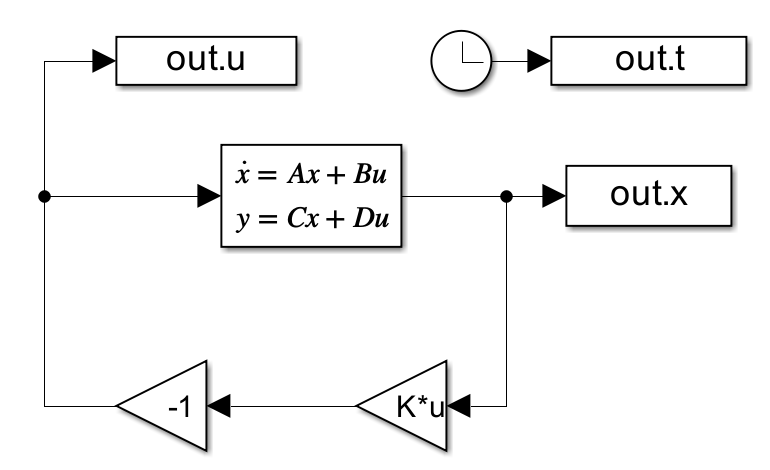
\includegraphics[width=0.3\linewidth]{Body/Images/LQR.png}
    \caption{Simulink implementation of the LQR controlled system.}
    \label{fig:lqr_simulink}
\end{figure}
\par By running the simulink for the initial condition $x_0 = \begin{bmatrix}
    0.1 & 0 & 0 & 0 & 0 
\end{bmatrix}$, it is possible to observe the evolution of the five states, converging to an equilibrium.
\begin{figure}[htbp]
    \centering
    
\includegraphics[width=0.4\linewidth]{Body/Images/Q6_states.pdf}
    \caption{Time-domain response of the LQR controller}
    \label{fig:lqr_simulink}
\end{figure}

\subsection{State Estimator Design - LQE}
\par Because the observed output only consists of $\alpha$ and $\beta$, it is necessary to design an estimator (Kalman Filter) that computes the entire state vector from the limited observed states. Since the system is observable, it is guaranteed that the state vector can be reconstructed by observing outputs $\alpha$ and $\beta$ over an interval of time. 

\par The estimated state model is given by:
\begin{equation} \label{eq:estimator_dyn}
    \dot{\hat{x}} = A \hat{x} + Bu + L(y - C \hat{x})
\end{equation}

\par The observer adds its own dynamics to the overall system, governed by the eigenvalues of $A - LC$. To compute the optimal estimator gain $L$, we consider the process noise covariance matrix $Q_r$ and the measurement noise covariance matrix $R_r$. The ratio of $Q_r$ to $R_r$ indicates how much the estimator trusts the physical measurements versus the mathematical model's predictions. High values in $Q_r$ paired with low values in $R_r$ indicate that the system should trust the incoming sensor measurements more.

\par The estimator gain $L$ is obtained via the expression $L = P C^T R_r^{-1}$, where the matrix $P$ (the error covariance) is found by solving the Continuous Algebraic Riccati Equation (CARE):

\begin{equation}
A P + P A^T - P C^T R_r^{-1} C P + G Q_r G^T = 0
\end{equation}
\par In the present work, we computed the optimal estimator gain by resorting to MATLAB's \texttt{lqe()} function.

\subsection{Baseline LQG Simulation}
\par By combining the LQR controller with the LQE observer, we create a Linear Quadratic Gaussian (LQG) controller. In this architecture, the estimated states are fed to the control law, which then computes the inputs to the plant. By combining Equation \ref{eq:lqr_cost} with Equation \ref{eq:estimator_dyn}, it is possible to arrive at the unified model for the controller block:

\begin{gather}
\dot{\hat{x}} = (A - BK - LC)\hat{x} + Ly, \\
u(t) = -K\hat{x}(t).
\end{gather}

\par The implementation of the observer paired with the controller—featuring the dynamic matrix $A - BK - LC$, input matrix $L$, and output matrix $-K$—led us to the following Simulink block diagram implementation:

\begin{figure}[htbp]
    \centering
    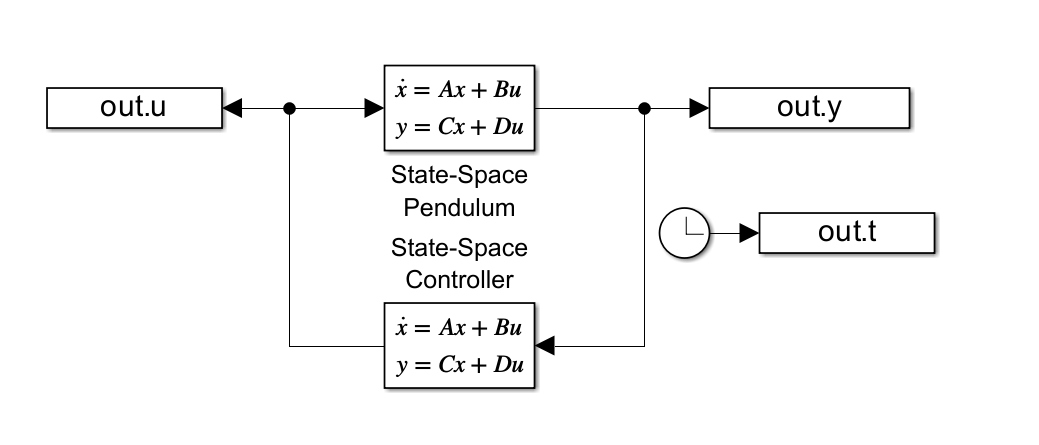
\includegraphics[width=0.4\linewidth]{Body/Images/LQE.png}
    \caption{Simulink implementation of the complete LQG system (Estimator + Controller).}
    \label{fig:lqg_simulink}
\end{figure}

\par By running the simulink with the initial condition $x_0 = \begin{bmatrix}0.1 & 0 & 0 & 0 & 0 \end{bmatrix}$, it is possible to obtain the evolution of the $\alpha$ and $\beta$ states, as well as the voltage $u$ outputed to the plant.

\begin{figure}[htbp]
    \centering
    \begin{subfigure}[b]{0.4\textwidth}
        \centering
        
\includegraphics[width=\textwidth]{Body/Images/Q8_angles.pdf}
        \caption{Evolution of states $\alpha$ and $\beta$}
        \label{fig:bode_alpha}
    \end{subfigure}
\hspace{0.05\textwidth}%
    \begin{subfigure}[b]{0.4\textwidth}
        \centering
        
\includegraphics[width=\textwidth]{Body/Images/Q8_voltage.pdf}
        \caption{Evolution of the output $u$}
        \label{fig:bode_beta}
    \end{subfigure}
    \label{fig:bode_plots_combined}
\end{figure}
\par It is possible to observe that both states are tracking the reference, with some minor overshoot. At this stage, it became paramount to understand the influence $Q_r$ and $R_r$ had on the response of the system. It is noted that multiplying $Q_r$ and $R_r$ by a constant $K$ does not influence the system response. This is because any multiplying constant in the cost function \eqref{eq:lqr_cost} can be factored out of the integral and does not change the optimal gain $K$. Consequently, only the relative weighting between $Q_r$ and $R_r$ determines the trade-off between minimizing state deviations and minimizing control effort.
\par Therefore, we varied the values of ${Q_r}_1$ and ${Q_r}_3$\footnote{To improve readibility, we adopted the convention of refering to entries of the $Q_r$ matrix based on the state they influence. For example ${Q_r}_1 = Q_r(\alpha)$ and ${Q_r}_3 = Q_r(\beta)$} with a fixed $R_r$ and vice-versa, in order to understand their effect on the system.
\begin{figure}[htbp]
    \centering
    \begin{subfigure}[b]{0.4\textwidth}
        \centering
        
\includegraphics[width=\textwidth]{Body/Images/Q9_Qr_alpha.pdf}
        \caption{Evolution of states $\alpha$ and $\beta$}
        \label{fig:Qr_alpha}
    \end{subfigure}
\hspace{0.05\textwidth}%
    \begin{subfigure}[b]{0.4\textwidth}
        \centering
        
\includegraphics[width=\textwidth]{Body/Images/Q9_Qr_beta.pdf}
        \caption{Evolution of the output $u$}
        \label{fig:Qr_beta}
    \end{subfigure}
    \label{fig:bode_plots_combined}
    \caption{Effect of $Q_r$ on the evolution of states $\alpha$ and $\beta$}
\end{figure}


\par From Figures \ref{fig:Qr_alpha} and \ref{fig:Qr_beta}, it can be observed that increasing the weighting associated with $Q_r(\alpha)$ leads to a reduction in both the overshoot and settling time of the states $\alpha$ and $\beta$. This indicates that placing a higher penalty on deviations of $\alpha$ results in a faster and more well-damped overall system response. 

\par Conversely, increasing the weighting $Q_r(\beta)$ produces a different effect: while it reduces the overshoot of state $\beta$, it tends to increase both the overshoot and settling time of state $\alpha$. This highlights the coupling between the system states and illustrates the trade-off inherent in selecting the weighting matrices.

\par We also analyzed the influence of the control weighting matrix $R_r$ while keeping $Q_r$ fixed.
\newpage
\begin{figure}[htbp]
    \centering
    
\includegraphics[width=0.5\linewidth]{Body/Images/Q9_Rr.pdf}
    \caption{Influence of $R_r$ on the system response.}
    \label{fig:Rr_LQG}
\end{figure}

\par From Figure \ref{fig:Rr_LQG}, it is evident that decreasing $R_r$ reduces both the overshoot and the settling time. This occurs because a smaller $R_r$ penalizes the control effort less, allowing the controller to act more aggressively and respond faster to deviations from the reference.